\documentclass{beamer}
\usepackage{etoolbox}\newtoggle{printable}\togglefalse{printable}
\usetheme{CambridgeUS}
\usepackage{listings}
\usepackage{algpseudocode}
\pdfmapfile{+sansmathaccent.map}
\graphicspath{ {Images/} }

\title{Comp240 Business Presentation}
\author{Alastair Rayner}
\date{\today}

\begin{document}

\maketitle


% ////////////////// TARGET AUDIENCE
\begin{frame}{About the Product}
	The product I have been working on is a lobby system for the BA team Firelock. \pause
	 
	However the product as a whole is the game being developed by the BA team. \pause
	
	This presentation will aim to address whether there is an audience for the game and which marketing strategy we believe to be the best for this product. \pause
\end{frame}


\begin{frame}{What is the target audience for this product?}		
	\textbf{What is the target audience for this product?} \pause
		\begin{itemize}
			\item One target audience for this product would be people who like to play video games with their friends, especially at LAN parties etc. \pause
			\item Another would be players who like strategy games such as Valkyria Chronicles and Frozen Synapse. \pause
				\begin{itemize}
					\item Both of these games have an owner base of around 700,000 players. \pause
					\item Valkyria Chronicles has sold a total of 1.3 million copies according to SteamSpy. \pause
				\end{itemize}	
			\item The demographic for the game would be males and females in the age range of about 12+.  \pause
				\begin{itemize}
					\item This demographic may not have a lot of disposable income, however they may have a lot of spare time. \pause
					\item They may also be interested in merchandise.
				\end{itemize}	
		\end{itemize}
\end{frame}

\begin{frame}{How lucrative is the target audience for this product?}
	\begin{itemize}
		\item There are very few competing games in this game genre \pause
		\item There is a large fairly new market for multiplayer games \pause
		\item This market in its current state is quite niche \pause
		

	\end{itemize}
\end{frame}

\begin{frame}{How to market effectively to the target audience}
	\begin{itemize}
	\item To appeal to the young target audience the game is intended to be sold at a relatively low cost in comparison to it's competitors \pause
	\item The marketing will focus on it's unique gameplay and multiplayer aspects \pause
	\end{itemize}	
	
	\center{\textbf{Additional marketing strategies:}}
	\begin{itemize}
		\item There are plans to create 3D printed in game items as merchandise that can be sold along side the game \pause
		\item These 3D items would be some of the in-game runes that players use \pause
		\item These items can be sent out to streamers and content creators to raise awareness of the game \pause
		\item This would promote the game and increase revenue \pause
		\item Having a strong social media presence \pause
	\end{itemize}
	
	
\end{frame}

% ///////////////////// POTENTIAL RISKS
\begin{frame}{Competitors and other risks}
	\center{\textbf{Potential Risks}}
	\begin{itemize}
		\item Change in market size \pause
		\item Miscalculating the product pricing (i.e. Pricing doesn't match the value as perceived by the customers \pause
		\item A new competitor enters the market \pause
		\item lots more.. \pause
	\end{itemize}
	\center{\textbf{Change in market size}}
	\begin {itemize}
	\item The market for this type of game has been around for while, as similar games such as Frozen Synapse was released in 2011. \pause
	\item This means that the market has been open for a while. \pause
	\item Furthermore steamspy stats show that the similar games have an active player base. \pause
	\end{itemize}
	
	
	
	
\end{frame}

\begin{frame}{Competitors and other risks}
	As this game has a rare hybridized tactical first person gameplay, this sets the game apart from most of the competition. 
	\center{\textbf{Comparative games}}
	\begin{itemize}
		\item Renowned Explorers: International Society
		This is a successful turn based strategy game that was produced by a team of a similar size. \pause
		\begin{itemize}
			\item This game made roughly \pounds 2,356,637 in sales. \pause
		\end{itemize}
		
		\item Valkyria Chronicles
		This game had a slightly larger studio size, however their game is the best comparison in relation to gameplay. \pause
		\begin{itemize}
			\item This game made roughly \pounds 13,200,913 in sales. \pause
		\end{itemize}
		
		
		\item Frozen Synapse
		This game is a turn based strategy game that was developed by a team of 4 core developers. \pause
		\begin{itemize}
			\item This game made roughly \pounds 6,725,052 in sales. \pause
		\end{itemize}
	\end{itemize}
\end{frame}

\begin{frame}{Similar Games}
	\center{SimilarGames}
	\par
	\center{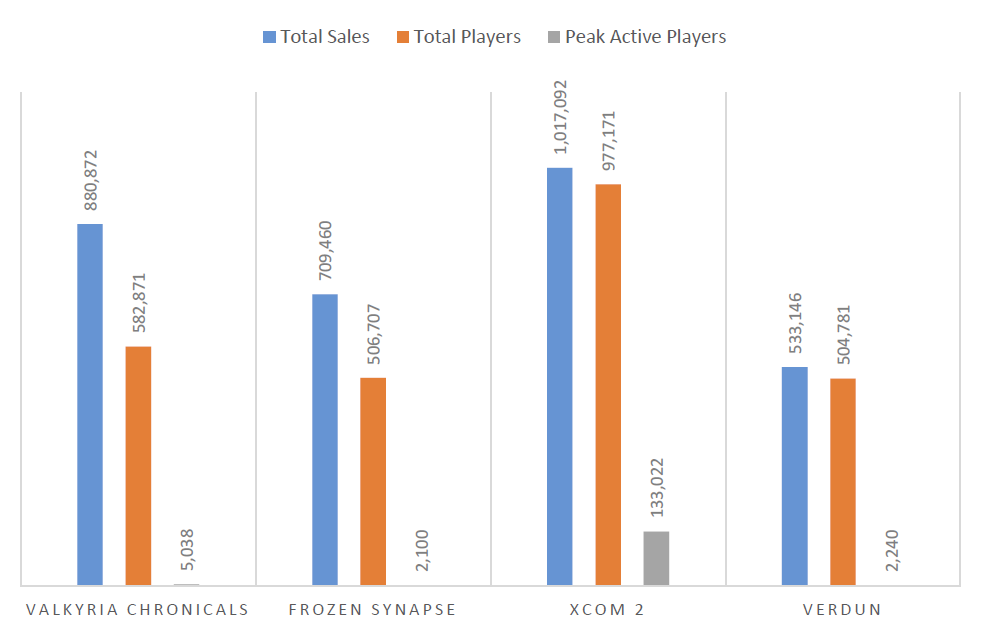
\includegraphics[width=8cm]{SimilarGames}}
\end{frame}


% ////////////////////////////// FEASIBILITY OF SUCCESS
\begin{frame}{Marketing Strategies}		

	Steam will be the primary distributor
\end{frame}

\begin{frame}{Financial Breakdown}
\center{Financial Breakdown}
	\par
	\center{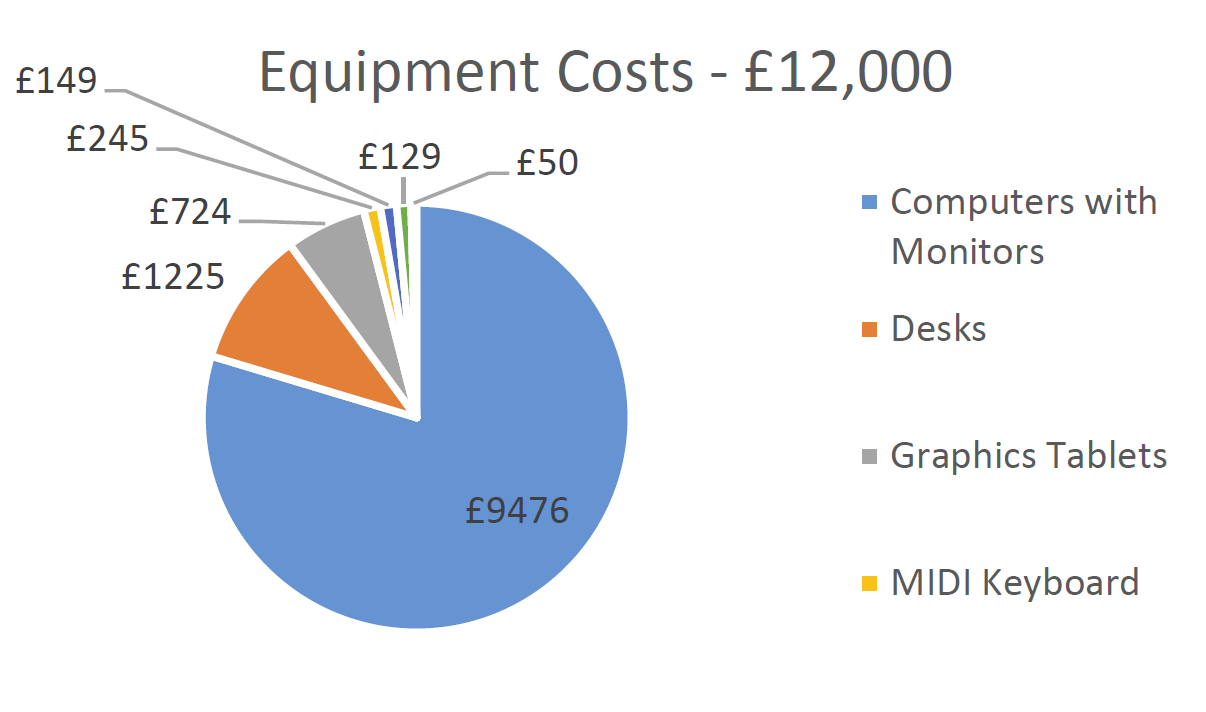
\includegraphics[width=8cm]{Finances}}
\end{frame}






% ////////////////////////// HOW TO EFFECTIVELY MARKET THIS TO THE AUDIENCE (Reference firelock marketing plan0




















\begin{frame}{Scope}
	\begin{itemize}
		\item Unity has quite a high level networking architecture already built in it.  \pause
		\item This meant that I didn't have to program very low level networking stuff and worry about security etc. \pause
		\item This made the scope of this component manageable for this time-frame. \pause
		\item However there is still a lot to be improved upon.
	\end{itemize}
\end{frame}

\begin{frame}{Images of the Lobby GUI}
	\begin{itemize}
		\item Lobby Menu. \pause
		\item 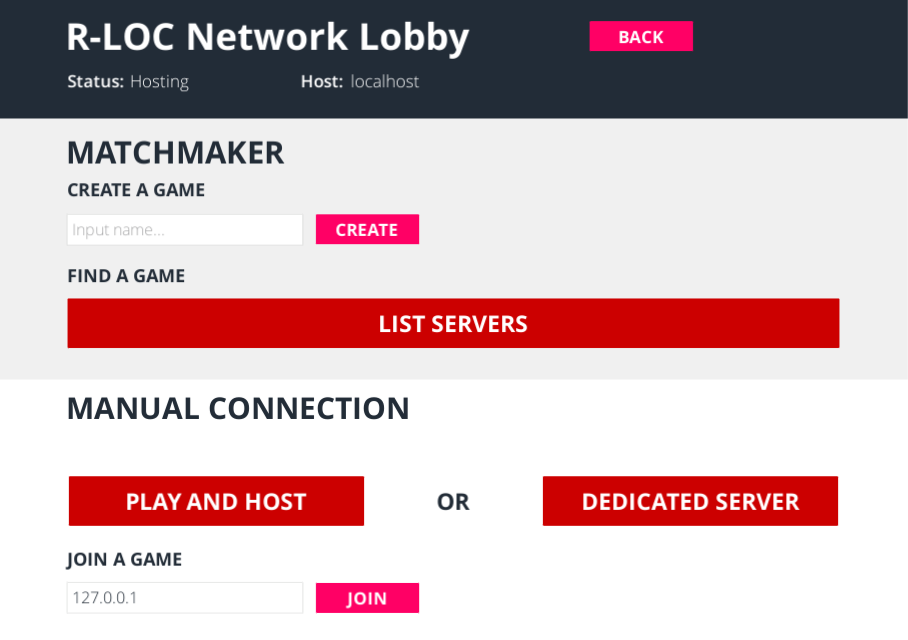
\includegraphics[width=8cm]{LobbyGUI} \pause
		\item Currently the Online Matchmaking isn't working.
	\end{itemize}
\end{frame}

\begin{frame}{Images of the Lobby GUI}
	\begin{itemize}
		\item Lobby Setup \pause
		\item 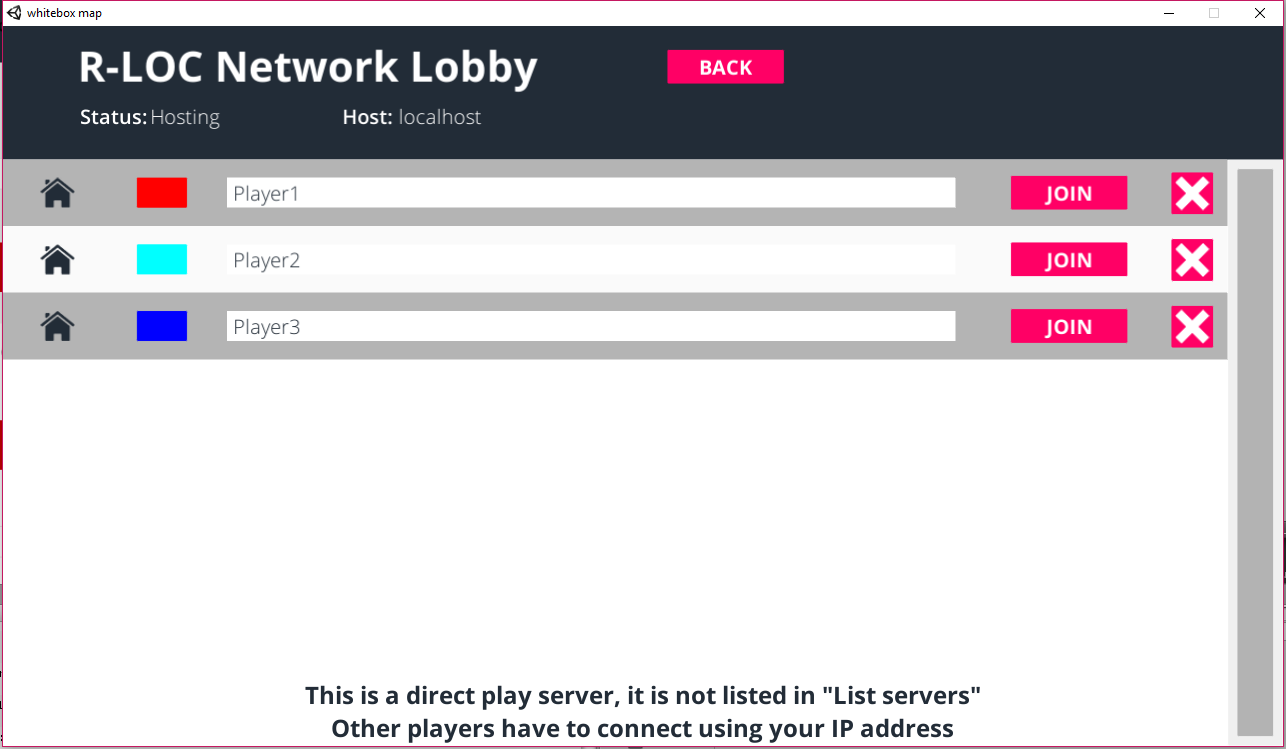
\includegraphics[width=8cm]{LobbySetup}
	\end{itemize}
\end{frame}

\begin{frame}{Networking Video Demo}
	\begin{center}
	Demo of working lobby and networked player movement.
	\par
		\url{https://www.youtube.com/watch?v=fUtDHb1e6x8&feature=youtu.be}
	\end{center}
\end{frame}

\begin{frame}{Moving Forward into Production}
	\begin{itemize}
		\item Lobby Menu GUI improvements. \pause
		\item Aim to get online matchmaking working. \pause
		\item Player is able to choose different types of units and select a map.
	\end{itemize}
\end{frame}
\begin{frame}{Questions?}
\begin{center}
\textbf{Questions?}
\end{center}
\end{frame}

\end{document}
